\documentclass[12pt]{article}
\usepackage{scrextend}
\usepackage[utf8]{inputenc}
\usepackage[polish]{babel}
\usepackage[T1]{fontenc}%polskie znaki
\usepackage[utf8]{inputenc}%polskie znaki
\usepackage[a4paper,left=0.42in,right=0.42in,top=0.25in,bottom=0.5in,noheadfoot]{geometry}
\usepackage{float}
\usepackage{enumitem}
\usepackage{hyperref}
\usepackage{graphicx}
\usepackage{tabulary}
\usepackage{etoc}
\usepackage[normalem]{ulem} 
\usepackage{tikz}
\usepackage[bf]{caption}
\usepackage{listings}
\usepackage{dirtytalk}
\usepackage{microtype}
\usepackage{graphicx}
\usepackage{setspace}
\usepackage{lmodern}
\usepackage{fancyhdr}
\usepackage{lastpage}
\usepackage{amsmath}
\renewcommand{\baselinestretch}{1.75}
\pagestyle{fancy}

\setlength{\parindent}{0pt}
\setlength{\parskip}{0pt}
\setstretch{1.75}
\renewcommand{\headrulewidth}{0pt}
\fancyhf{}
\lhead{}
\lfoot{
  \hrule
  \textsc{Projekt Akceleracja obliczeń w przetwarzaniu danych}
}
\rfoot{
  \hrule
  \textsc{strona \thepage / \pageref{LastPage}}
}
\usepackage{listings}
\usepackage{xcolor}
 
\definecolor{codegreen}{rgb}{0,0.6,0}
\definecolor{codegray}{rgb}{0.5,0.5,0.5}
\definecolor{codepurple}{rgb}{0.58,0,0.82}
\definecolor{backcolour}{rgb}{0.97,0.97,1.0}
 
\lstdefinestyle{mystyle}{
    backgroundcolor=\color{backcolour},   
    commentstyle=\color{codegreen},
    keywordstyle=\color{magenta},
    numberstyle=\tiny\color{codegray},
    stringstyle=\color{codepurple},
    basicstyle=\fontsize{11}{9}\ttfamily,%\footnotesize,
    breakatwhitespace=false,         
    breaklines=true,                 
    captionpos=b,                    
    keepspaces=true,                 
    numbers=left,                    
    numbersep=5pt,                  
    showspaces=false,                
    showstringspaces=false,
    showtabs=false,                  
    tabsize=1,
    postbreak=\mbox{\textcolor{red}{$\hookrightarrow$}\space}
}
\renewcommand{\lstlistlistingname}{Spis listingów}\lstset{style=mystyle}


\graphicspath{images/}
\newgeometry{lmargin=2.0cm, rmargin=2.0cm, tmargin=2.0cm, bmargin=2.0cm}
\clubpenalty=9996
\widowpenalty=9999
\brokenpenalty=4991
\predisplaypenalty=10000
\postdisplaypenalty=1549
\displaywidowpenalty=1602

\title{ 
    \vspace*{55mm}
    \textsc{
        \textbf{Akceleracja obliczeń w przetwarzaniu danych\\Projekt}\\
        \large Wyszukiwanie słów w tekście z wykorzystaniem algorytmu Rabina-Karpa
        }
} 
\author{
\vspace{15mm}\\
Szymon Filipiak, 241309\\
Dawid Zawadzki, 241116\\
Wiktor Pieklik, 241282\\
\vspace{15mm}
}


\date{Wrocław, \today}
\begin{document}
\maketitle

\newpage
\setcounter{tocdepth}{2}
\localtableofcontents

\newpage
\listoffigures
\lstlistoflistings
\newpage

\section{Wstęp}
Rozwiązanie opisywanego projektu znajduje się w publicznym repozytorium \url{https://github.com/WiktorPieklik/GPU_Karp_Rabin}.
\subsection{Zakres i cel}
Celem naszego projektu jest poznanie technik oraz narzędzi do tworzenia oprogramowania wykonywalnego na kartach graficznych. Skupimy się na kartach firmy \textbf{NVIDIA} \cite{nvidia}. Wymaga to pozanania specyfiki architektury tych urządzeń oraz sposobu programowania w framework'u \textbf{CUDA} (Compute Unified Device Architecture) \cite{cuda}. Do realizacji naszych celów zaimplementujemy algorytm \textit{Karpa-Rabina}, dzięki któremu będziemy mogli poszukiwać zadanej frazy w zadanym tekście. Algorytm ten będzie zaimplementowany w dwóch wersjach:
\begin{itemize}
    \item na główny procesor \textbf{CPU},
    \item na procesor graficzny \textbf{GPU}.
\end{itemize}
Następnie przeprowadzimy serię testów w celu jakościowej oceny zastosowanych rozwiązań, na podstawie której ustalimy czy proces zrównoleglania przyniósł efekt w postaci skrócenia czasu wykonywania algorytmu. Przeprowadzimy także testy, które pomogą nam określić jak dobrze nasza implementacja algorytmu wykorzystuje możliwości \textbf{GPU}.
\section{Algorytm Rabina-Karpa}
\subsection{Opis}
Jest to algorytm przeszukiwania tekstu zaproponowany przez \textit{Richarda Karpa oraz Michaela Rabina} i przedstawiony światu w 1987 roku na łamach magazynu \textit{IBM Journal of Research and Development} w artykule \textit{Efficient randomized pattern-matching algorithms} \cite{rabin_karp_alg}.\\
Algorytm \say{naiwny} dla tego problemu oparty jest na porównywaniu szukanego wzorca z każdą pozycją w tekście, co w najgorszym przypadku cechuje się złożonością obliczeniową \textit{O(n*m)} (gdzie \textit{n} to długość szukanego wzorca, a \textit{m} to długość przeszukiwanego tekstu).
Alogrytm \textit{Rabina-Karpa} stanowi usprawnienie \say{naiwnego} podejścia poprzez wykorzystanie:
\begin{itemize}
    \item elementarnego pojęcia teorii liczb jakim jest przystawanie dwóch liczb modulo,
    \item funkcji haszującej \textit{$h(x_{i})$},
    \item funkcji obliczającej \say{kroczący} hasz (ang. \textit{rolling hash}) niskim kosztem  poprzez wyznaczenie \textit{$h(x_{i+1})$} na podstawie \textit{$h(x_{i})$}.
\end{itemize}
Kluczowa, dla algorytmu, jest interpretacja alfabetu $\sum$, która pozwala traktować tekst \textit{k} symboli jako liczbę \textit{k-cyfrową} w systemie o podstawie \textit{d} (gdzie \textit{$d = |\sum|$}). Interpretacja ta odbywa się za pomocą wyliczania wartości hasza dla zadanego podciągu przeszukiwanego tekstu. Wartość hasza obliczana jest za pomocą reguły \textit{Hornera}:
\[ hasz = wzorzec[n-1] + d(wzorzec[n-2] + d(wzorzec[n-3]) + \ldots + d(wzorzec[1] + d*wzorzec[0]) \ldots ))\]
W celu zapewnienia stałego czasu wykonywania operacji arytmetycznych podczas wyliczania wartości hasza dla dowolnie długich podciągów, stosuje się dzielenie modulo \textit{q}. Powszechną praktyką jest, aby wybrana liczba \textit{q} była liczbą pierwszą oraz aby wartość \textit{d*q} mieściła się w zakresie słowa maszynowego procesora, co zapewnia wykonanie wszystkich operacji arytmetycznych z pojedynczą precyzją.
Proces obliczania wartości \say{kroczącego} hasza został przedstawiony na rysunku \ref{fig:rolling_hash}.
\begin{figure}[H]
    \centering
    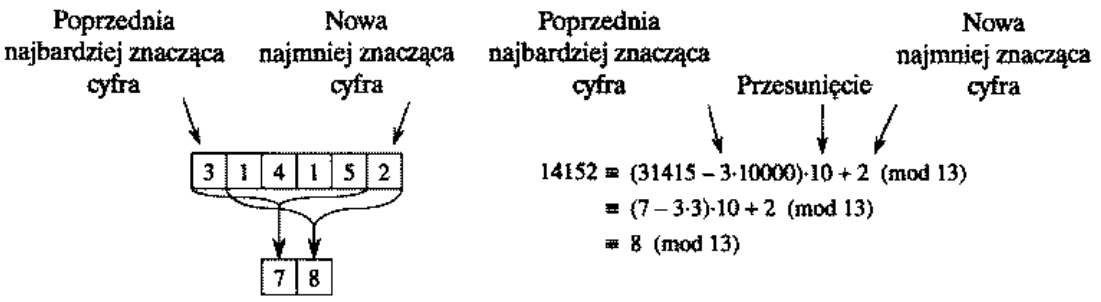
\includegraphics[width=\linewidth]{images/RollingHash.png}
    \caption{Schemat obliczania wartości \glqq kroczącego\grqq \space hasza \cite{cormen}}
    \label{fig:rolling_hash}
\end{figure}
Mając obliczone wartości funkcji haszującej dla wzorca i wybranego podzbioru tesktu możemy sprawdzić, czy następuje wystąpienie wzorca w tekście. Warto zaznaczyć, że samo porównanie wartości haszów nie wystarcza; kongruentność dwóch liczb nie implikuje ich równości. Jeżeli wartości haszy są sobie równe należy sprawdzić, czy wybrany pozdbiór tesktu i wzorzec to te same słowa. Natomiast, jeżeli wartości haszy nie są sobie równe należy zacząć liczenie \say{kroczącego} hasza dla następnej pozycji; jeżeli dwie liczby nie przystają do siebie modulo to na pewno nie są sobie równe.
\subsection{Cechy}
Algorytm cechuje się oczekiwaną złożonością czasową \textit{O(m+n)} oraz pesymistyczną złożonością czasową \textit{$O((m-n + 1)n) \approx O(m*n)$}. W implementacji algorytmu można podzielić szukany tekst na mniejsze fragmenty przy jednoczesnym zachowaniu założeń proponowanej metody (operacja fragmentaryzacji tekstu nie jest obarczona dużą złożonością czasową). Pomimo swojej sekwencyjnej natury, algorytm daje się w łatwy sposób zrównoleglić. 
\section{Implementacja}
\label{chapter:3}
\subsection{Wymagania funkcjonalne}
Użytkownik może:
\begin{itemize}
    \item podać ścieżkę do pliku będącego przeszukiwanym tekstem,
    \item podać przeszukiwany tekst w postaci ciągu znaków (parametr wywołania programu),
    \item podać szukany wzorzec,
    \item zobaczyć wystąpienia (lub ich brak) wzorca w tekście,
    \item przeprowadzić testy wydajności implementacji algorytmu dla danego pliku i danych wzorców.
\end{itemize}
\subsection{Wymagania niefunkcjonalne}
Implementowany program:
\begin{itemize}
    \item wykorzystuje technologię \textbf{NVIDIA CUDA},
    \item wykorzystuje narzędzie \textbf{CMake} do procesu kompilacji,
    \item pisany jest w języku programowania \textbf{C++20},
    \item korzysta z kompilatorów: \textbf{gcc} oraz \textbf{cygwin}
\end{itemize}

\newpage
\subsection{Architektura}
Ze względu na złożoność problemu, program został podzielony na mniejsze, niezależne moduły:
\begin{itemize}
    \item moduł odpowiedzialny za wczytywanie tekstu,
    \item moduł odpowiedzialny za dzielenie tekstu na mniejsze fragmenty,
    \item moduł obliczający wartości haszów,
    \item moduł odpowiedzialny za przeprowadzanie pomiarów wydajności działania programu,
    \item moduł główny, zarządzający działaniem całego programu.
\end{itemize}
Podział na moduły został zaprezentowany na rysunku \ref{fig:dir_structure}.
\begin{figure}[H]
    \centering
    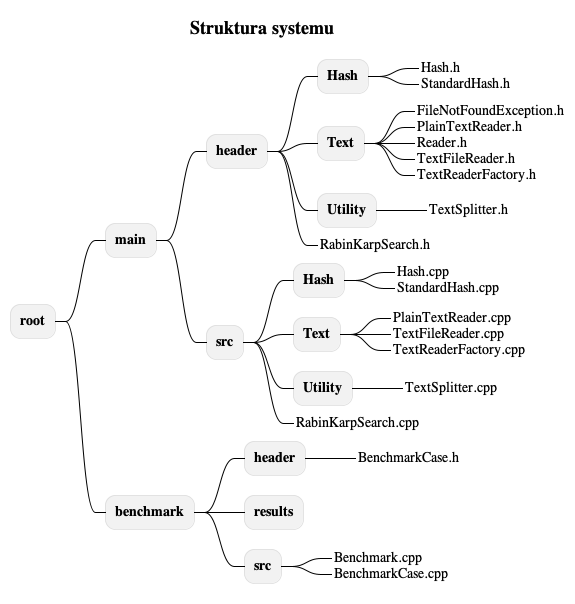
\includegraphics[scale=0.65]{images/uml/DirStructure.png}
    \caption{Struktura projektowanego systemu}
    \label{fig:dir_structure}
\end{figure}
Pomiędzy wymienionymi modułami występują zależności przedstawione na rysnku \ref{fig:rabin_karp_search}.
\begin{figure}[H]
    \centering
    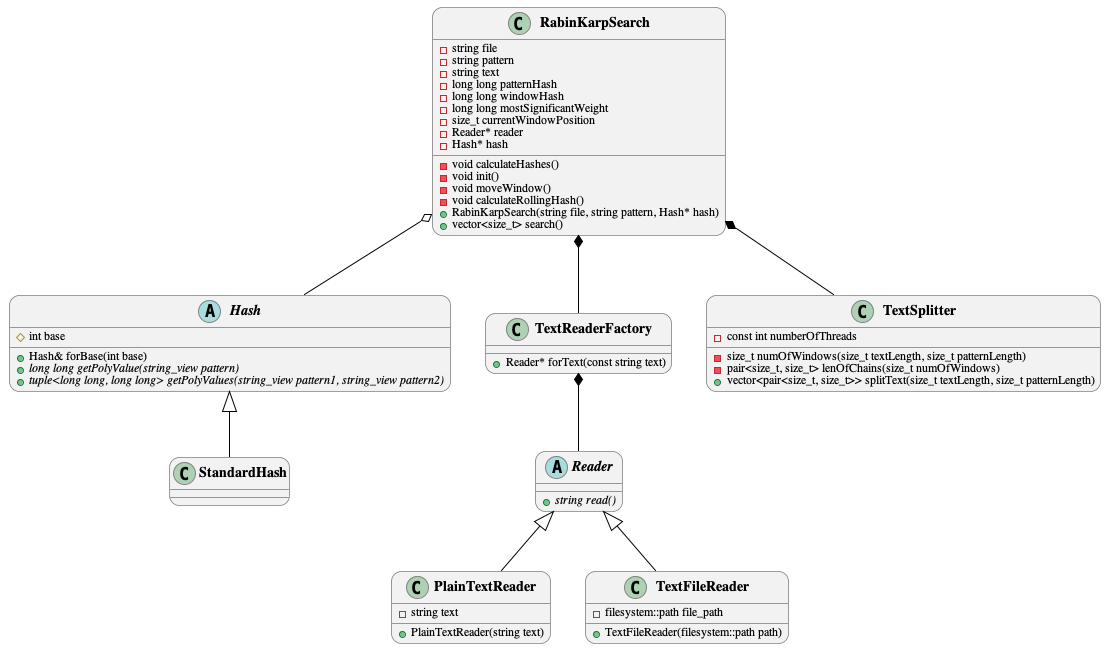
\includegraphics[width=\linewidth]{images/uml/RabinKarpSearch.png}
    \caption{Zależności pomiędzy modułami programu}
    \label{fig:rabin_karp_search}
\end{figure}
Na listingu \ref{lst:main_cpu} zaprezentowano przykładowe użycie modułu \textit{RabinKarpSearch} w wersji \textbf{CPU}. 
\begin{lstinputlisting}[language=C++, label=lst:main_cpu, caption=Przykładowe użycie modułu \textit{RabinKarpSearch} w wersji \textbf{CPU}]{listings/main_cpu.tex}
\end{lstinputlisting}

\subsection{Sposób równoleglenia operacji}
\label{subsec:parallelism}
Głównym aspektem równoleglenia implementacji algorytmu \textit{Rabina-Karpa} jest podział tekstu na zazębiające się podzbiory przeszukiwanego tekstu. W tym kontekście \textit{zazębiające się} oznacza, że wątki \textbf{GPU} analizują niezależnie od siebie i w niekontrolowanej kolejności określone podzbiory przeszukiwanego tekstu, symulując działanie \textit{x} niezależnych, sekwencyjnych instancji przeszukujących odpowiednio mniejszy fragment tekstu, który \say{nachodzi} na sąsiedni fragment tekstu. Sumarycznie, te \textit{x} sekwencyjnych instancji przeszukuje cały, zadany przez użytkownika, tekst. Proces podziału, na opisane fragmenty, został konceptualnie przedstawiony na rysunku \ref{fig:text_splitting}.
\begin{figure}[H]
    \centering
    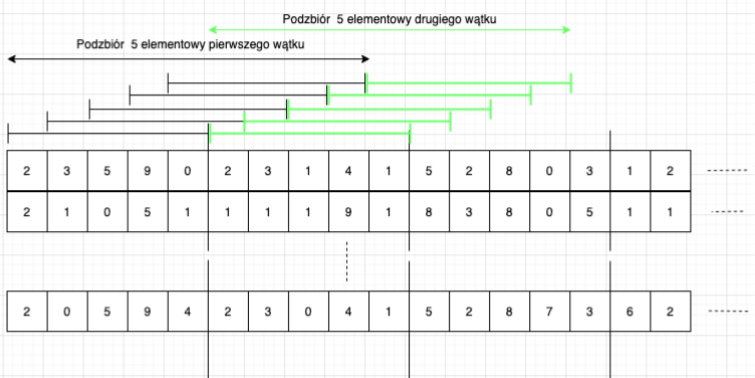
\includegraphics[width=\linewidth]{images/TextSplitting.png}
    \caption{Podział tekstu na zazębiające się fragmenty}
    \label{fig:text_splitting}
\end{figure}
Wiedząc, jak działa dzielenie tekstu, należy wydobyć taką liczbę fragmentów tekstu oraz dostosować długość pojedynczego fragmentu tak, aby każdy z wątków był równomierne obciążony i mógł przetworzyć możliwie jak największe fragmenty tekstu. Do tego celu proponujemy następujące rozwiązanie. 
\newpage
Niech dane będą: \textit{L} - długość przeszukiwanego tekstu, \textit{T} - liczba wątków, \textit{S} - długość szukanego wzorca, wtedy \textit{$C_i$} - długość fragmentu tekstu dla \textit{i-tego} wątku można określić zależnością:
\[
C_{i} = \begin{cases}
    \frac{L-S}{T} + 1& \text{dla i < (L - S) mod T}, \\
    \frac{L-S}{T}& \text{dla i $\geq$ (L - S) mod T}
\end{cases}
\]
Proces wykonywania się algorytmu z wykorzystaniem \textbf{GPU} został przedstawiony na rysnku \ref{fig:flow_chart}.
\begin{figure}[H]
    \centering
    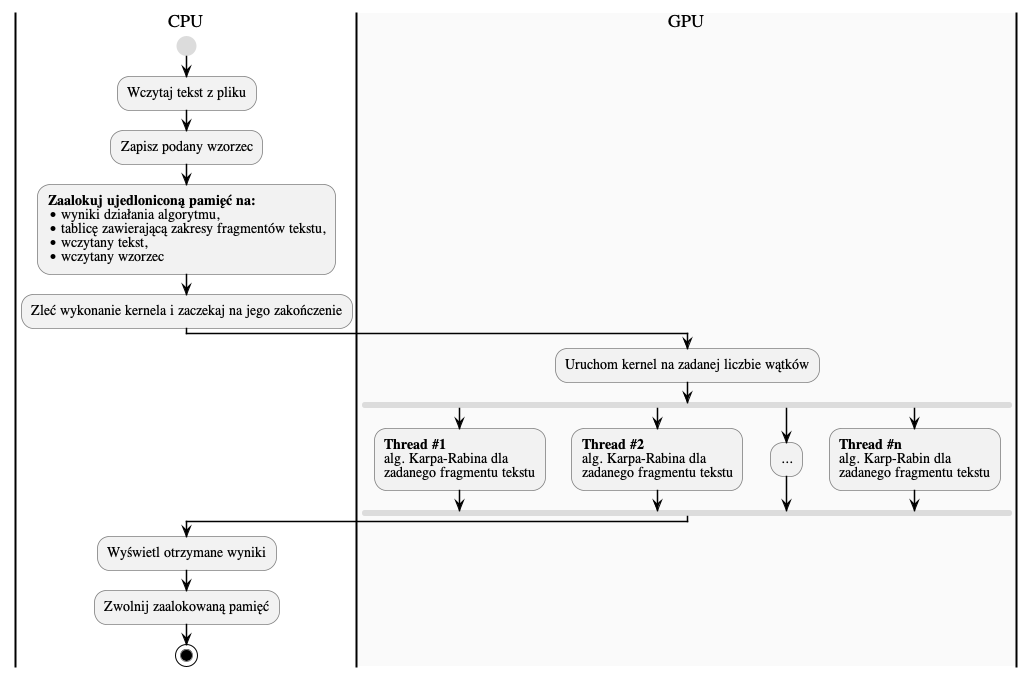
\includegraphics[width=\linewidth]{images/uml/FlowChart.png}
    \caption{Schemat działania programu dla wersji \textbf{GPU}}
    \label{fig:flow_chart}
\end{figure}

\newpage
Natomiast na listingu \ref{lst:main_gpu} przedstawiono przykładowe użycie modułu \textit{RabinKarpSearch} w wersji \textbf{GPU}.
\begin{lstinputlisting}[language=C++, label=lst:main_gpu, caption=Przykładowe użycie modułu \textit{RabinKarpSearch} w wersji \textbf{GPU}]{listings/main_gpu.tex}
\end{lstinputlisting}

\section{Pomiary wydajności}
Wydajność stworzonej implementacji algorytmu została przebadana na podstawie specjalnie stworzonego zestawu testów, który pozwolił porównać czas wykonywania się programu w wersji \textbf{GPU} do wersji działającej na \textbf{CPU}. Zaplanowano także pomiary uwzględniające przypadki optymistyczne i pesymistyczne dla algorytmu Rabina-Karpa w celu wykazania przyspieszenia działania programu w wersji zrównoleglonej, w każdym możliwym przypadku. 

\subsection{Parametry sprzętowe}
Pomiary zostały przeprowadzone na procesorze \textbf{Intel Core i5-9300H CPU 2.40GHz} oraz karcie graficznej \textbf{NVidia GeForce GTX 1050 3GB}.

\subsection{Różna długość przeszukiwanego tekstu}
Aby przeprowadzić badanie wygenerowano pliki tekstowe złożone z losowych znaków o różnych rozmiarach, a następnie zostały przeprowadzone pomiary, które zestawione są na rysunku \ref{fig:chart_1}.

\begin{figure}[H]
    \centering
    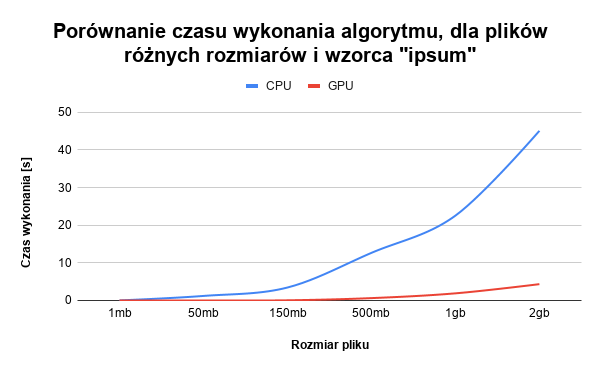
\includegraphics[width=\linewidth]{images/wykres41.png}
    \caption{Porównanie czasu wykonania obu wersji algorytmu, dla plików rożnych rozmiarów}
    \label{fig:chart_1}
\end{figure}

Na załączonym wykresie można zauważyć znaczną przewagę symultanicznej wersji algorytmu. Dla pliku o rozmiarze 2GB otrzymano aż 40 sekund zysku. Rysunek \ref{fig:chart_1} pokazuje również, że charekterystka zależności czasu wykonania od rozmiaru pliku dla algorytmu działającego na \textbf{GPU} rośnie wolniej od charakterystyki dla algorytmu działającego na \textbf{CPU}.

\subsection{Różna długość szukanego wzorca}

Pomiary dla wzorca o różnej długości dla pliku o rozmiarze 500MB zostały przeprowadzone w celu sprawdzenia, czy długość szukanej frazy nie ma drastycznego wpływu na czas wykonania algorytmu. Niestety, charakterystyka użytego algorytmu haszującego nie pozwoliła na wykonanie pomiarów dla wzorca posiadającego więcej niż 50 znaków, ze względu na przekroczenie maksymalnego zakresu zmiennej typu \textbf{long long int}. Uzyskane wyniki zostały przedstawione na rysunku \ref{fig:chart_2}.


\begin{figure}[H]
    \centering
    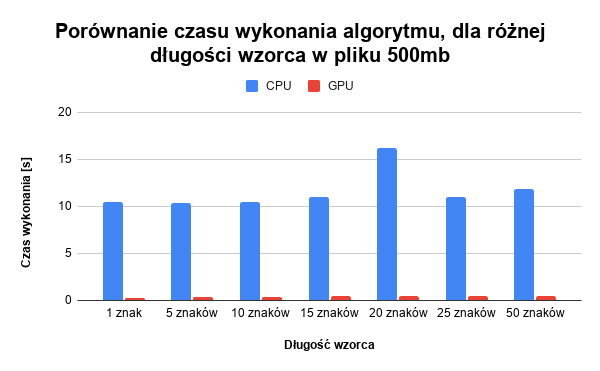
\includegraphics[width=\linewidth]{images/wykres42.png}
    \caption{Porównanie czasu wykonania obu wersji algorytmu, dla wzorca różnej długości}
    \label{fig:chart_2}
\end{figure}

Analizując wyniki przedstawione na rysunku \ref{fig:chart_2} można stwierdzić, że pomiary czasu wykonywania algorytmu dla wzorców o długości mniejszej niż 20 znaków oscylują wokół 10 sekund. Dla wzorca o długości 20 znaków obserwuje się najdłuższy czas wykonania algorytmu na \textbf{CPU}. Wynika to z wyboru specyficznego wzorca, którego hasz częściej zgadzał się z haszem porównywanych okien. W takim przypadku wartości funkcji haszującej były jednakowe, co skutkowało potrzebą wykonania dodatkowych operacji porównania. Dla pozostałych pomiarów obserwowalny jest nieznaczy wzrost czasu wykonywania wraz ze wzrostem długości wzorca.\\
Pomimo braku możliwości zbadania algorytmu dla dłuższych ciągów znaków, posiada on pewne cechy, które pozwalają antycypować jak będzie się zachowywał. W oparciu o wzór przedstawiony w podrozdziale \ref{subsec:parallelism} nie można dopuścić do przypadku, w którym \textit{$C_i$} \text{<} \textit{S}. Jedynym sposobem, który pozwala tego uniknąć, jest odpowiednie zmniejszenie liczby wątków, na których wykonywany jest algorytm. W najgorszym przypadku może to skutkować wykonywaniem całego programu w obrębie tylko jednego warp'a. Oznacza to, że potencjał karty graficznej byłby wykorzystany w małym procencie i prawdopodobnie uzyskanie gorszych rezultatów niż w przypadku \textbf{CPU}.

\subsection{Optymistyczne i pesymistyczne przypadki}

Dla algorytmu \textit{Rabina-Karpa} istnieją przypadki optymistyczne, których złożoność obliczeniowa wynosi \textit{O(m+n)} oraz pesymistyczne, których złożoność obliczeniowa wynosi \textit{$O(m*n)$}. Przypadek optymistyczny to taki, w którym hasz każdego porównywanego okna nie jest równy haszowi wzorca, co skutkuje brakiem operacji porównania tekstu, a więc również krótszym czasem wykonania. Natomiast pesymistyczne przypadki to takie, gdzie hasz każdego porównywanego okna jest równy haszowi wzorca co skutkuje, że porównywanie \say{znak po znaku} następuje za każdym razem. Taka sytuacja ma negatywny wpływ na wydajność. Przygotowane zestawy danych pozwoliły na zbadanie oraz porównanie czasu wykonania algorytmu dla takich przypadków, a uzyskane wyniki przedstawiono na rysunku \ref{fig:chart_3}.

\begin{figure}[H]
    \centering
    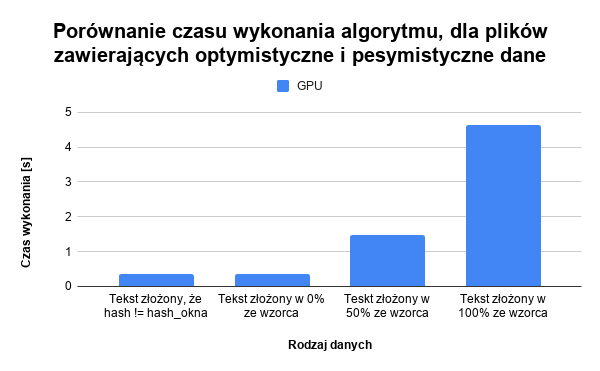
\includegraphics[width=\linewidth]{images/wykres43.png}
    \caption{Wyniki wersji na \textbf{GPU}, dla optymistycznych i pesymistycznych przypadków}
    \label{fig:chart_3}
\end{figure}

Na powyższym wykresie można zauważyć, że w przypadku pesymistycznym, algorytm działa wolniej aż 9-krotnie, niż dla przypadków optymistycznych. Widać również, że dla tekstu, w którym wystąpienie szukanego wzorca wynosiło \textit{$0\%$} otrzymano wyniki bardzo przybliżone do wyników dla danych optymistycznych. Spowodowane jet to niską częstotliwością występowania okien, których hasz zgadza się z haszem szukanego wzorca.
\section{Optymalizacja programu}
W celu określenia wydajności programu w kontekście wykorzystania dostępnych zasobów karty graficznej użyto narzędzia \textbf{NVIDIA Nsight Compute}. Pozwala ono na zbieranie wielu danych odnośnie wykonywanego programu i jego interakcji z kartą graficzną. Wiedza o tych interakcjach jest podstawą do prób optymalizacji programu. Wyniki przedstawiono poniżej.

\subsection{Wyniki programu profilującego}

Podstawowym badaniem przeprowadzanym przez narzędzie jest \textbf{GPU Speed Of Light}. To ogólne porównanie wykorzystanych zasobów obliczeniowych i pamięciowych do teoretycznego maximum parametru dla danej karty graficznej.\\
Na rysunku \ref{fig:speed_of_light} przedstawiono wyniki z działania tego narzędzia dla naszego programu.
\begin{figure}[H]
    \centering
    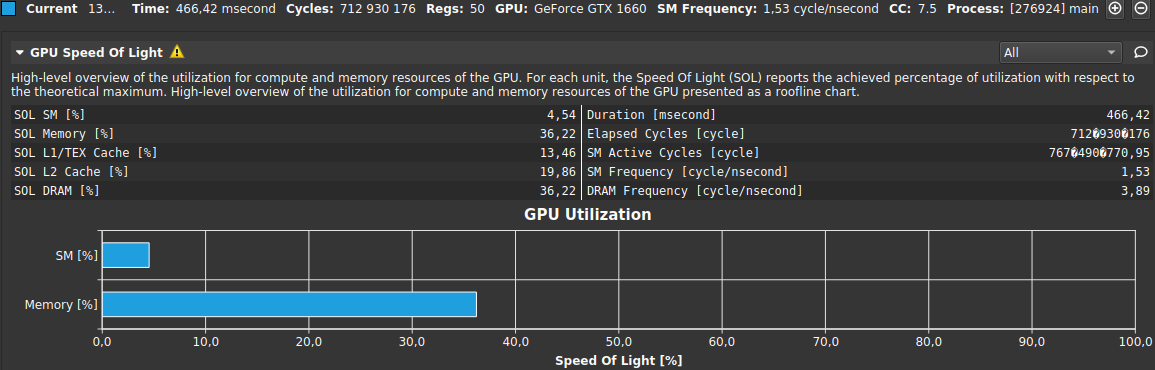
\includegraphics[width=\linewidth]{images/SpeedOfLight.png}
    \caption{Wyniki badania \textbf{GPU Speed Of Light}}
    \label{fig:speed_of_light}
\end{figure}
Widać, że wykorzystanie możliwości obliczeniowych karty graficznej to w tym przypadku ok. 4\%, a pamięci ok. 35\%.\\
Natomiast na rysunku \ref{fig:sm_analisys} przedstawiono treść ostrzeżenia znajdującego się w sekcji \textbf{Speed Of Light} oraz wyniki dokładniejszej analizy obciążenia procesorów strumieniowych.
\begin{figure}[H]
    \centering
    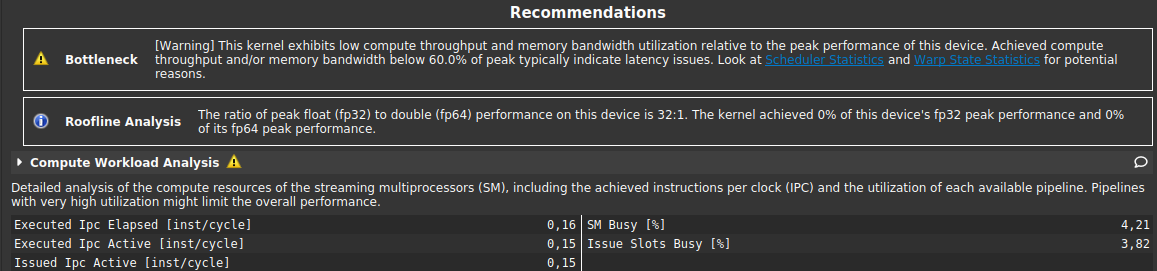
\includegraphics[width=\linewidth]{images/SMAnalysis.png}
    \caption{Wyniki badania \textbf{Compute Workload Analysis}}
    \label{fig:sm_analisys}
\end{figure}
Powyższe wyniki wskazują na to, że karta nie pracuje z pełną wydajnością. Wyniki tego badania jednak nie wskazują jasno, gdzie tracona jest skuteczność implementacji. Ostrzeżenie podpowiada, by sprawdzić wyniki badaniań \textbf{Scheduler Statistics} i \textbf{Warp State Statistics}. 

\begin{figure}[H]
    \centering
    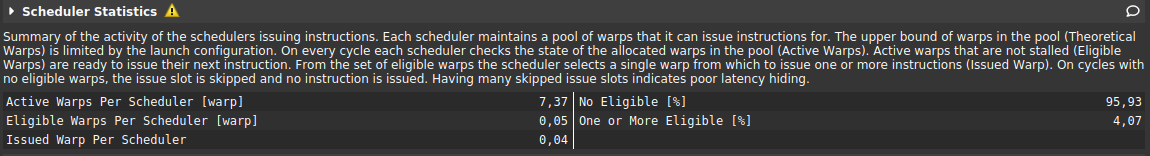
\includegraphics[width=\linewidth]{images/Scheduler.png}
    \caption{Wyniki badania \textbf{Scheduler Statistics}}
    \label{fig:scheduler}
\end{figure}

Na grafice \ref{fig:scheduler}. widać niskie wartości dwóch ostatnich pozycji w lewej kolumnie wyników, co wskazuje na małą średnią liczbę aktywowanych warp'ów na jeden cykl (\textit{Eligible Warps Per Scheduler}, \textit{Issued Warps Per Scheduler}). Liczba warp'ów znajdujących się w stanie aktywnym jest za to wysoka (dla tej architektury karty maksymalna ich liczba wynosi 8). Potwierdzają to także statystyki z prawych kolumn mówiące o wysokiej niedostępności warp'ów (\textit{No Egible} - 96\%). Takie wyniki mogą wskazywać na duże problemy związane z opóźnieniem dostępu do pamięci.

Wyniki badania \textbf{Warp State} pokazują także dość dużą średnią liczbę cykli na wykonaną jedną instrukcję programu.

\begin{figure}[H]
    \centering
    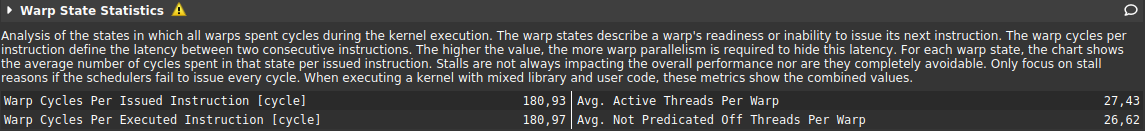
\includegraphics[width=\linewidth]{images/WarpState.png}
    \caption{Wyniki badania \textbf{Warp State Statistics}}
    \label{fig:warps}
\end{figure}

\subsection{Wnioski profilowania}

Powyższe wyniki wskazują jednoznacznie na słabe wykorzystanie przez program mocy \textbf{GPU}. Przyczyną tego jest potrzeba dostępu do różnych obszarów pamięci dla każdego wątku. Dostęp do pamięci globalnej (w niej przechowujemy przeszukiwany tekst) odbywa się dla każdego wątku pobierając zawsze 128-bitowy fragment pamięci. Jest on później zapisywany w pamięci współdzielonej, do której mają dostęp wątki z jednego warp'a. Jeśli kolejne wątki potrzebują danych ułożonych w pamięci sekwencyjne, to liczba dostępów do pamięci globalnej jest drastycznie mniejsza. Zastępowana jest dużo szybszym dostępem do pamięci współdcielonej, która ma czas dostępu porównywalny z czasem dostępu do rejestrów. Dużą liczbę odwołań do pamięci globalnej potwierdzają także dodaktowe komunikaty profilera, po wykonywaniu analizy wywołań poszczególnych instrukcji kodu. 

\begin{figure}[H]
    \centering
    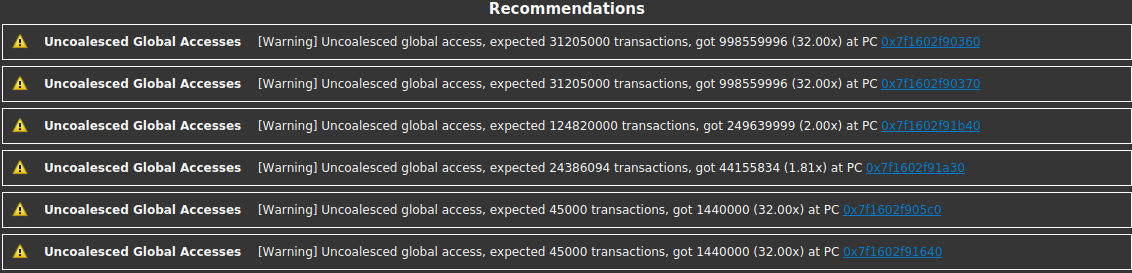
\includegraphics[width=\linewidth]{images/Warnings.png}
    \caption{Rekomendacje programu profilującego w sekcji \textbf{Source Counters}}
    \label{fig:warnings}
\end{figure}

Ostrzeżenia te mówią, o spodziewanej, optymistycznej liczbie dostępów do pamięci globalnej dla zadanej linii kodu, a rzeczywistym stanem. Różnice często są, w naszym przypadku, 32 krotne. Bezpośrednim powodem tego problemu jest struktura naszego programu. Kolejne wątki muszą mieć dostęp do stosunkowo odległych fragmentów przeszukiwanego tekstu. Aby zachować jednak charakter algorytmu Rabina-Karpa, tj.: obliczanie funkcji haszującej z wykorzystaniem wartości tejże funkcji dla poprzedniego okna tekstu, trzeba zachować przynajmniej lokalną sekwencyjność wykonywanego algorytmu. Najlepiej działa on, gdy sekwencje wyszukiwanych  Można się zastanowić, czy utrata wydajności spowodowana takim podejściem do problemu jest większa niż zyski spowodowane szybkim obliczaniem funkcji haszującej. Odpowiedzią na to pytanie byłoby porównanie naszej wersji algorytmu do równoległego, \say{naiwnego} przeszukiwania tekstu. W przypadku badania wykonanego dla optymistycznych przypadków, algorytm wykazał nawet 9-krotne przyspieszenie (rys. \ref{fig:chart_3}) w stosunku do przypadków pesymistycznych, dla których rozwiązanie degeneruje się do przeszukiwania \say{naiwnego}. Jeżeli implementacja \say{naiwna} miałaby być szybsza, musiałaby wykorzystywać zasoby karty graficznej przynajmniej kilkukrotnie lepiej niż obecny program.

%DAAAAAAMN!%
\section{Podsumowanie}
Na podstawie uzyskanych wyników oceniamy, że próby przyspieszenia implementacji algorytmu przez zrównoleglenie się powiodły. Widać to wyraźnie na wykresach \ref{fig:chart_1}. i \ref{fig:chart_2}. Uzyskano dość dużą różnice czasu wykonywania programu przeznaczonego na \textbf{GPU} w stosunku do wersji \textbf{CPU}. Przyspieszenie było nawet 100-krotne  dla plików o rozmiarze 500 MB. Nie oznacza to jednak, że udało nam się osiągnąć pełnie możliwości przyspieszenia tego algorytmu. Wyniki analizy programu w wersji \textbf{GPU} przez narzędzia do optymalizacji algorytmu wykazują jego niską skuteczność w wykorzystaniu zasobów sprzętowych. 
Otrzymane wyniki pozwoliły nam lepiej zrozumieć mechanizmy działania, zalety i ograniczenia programowania na akceleratory graficzne. Szczególnie pouczająca okazała się analiza wyników narzędzia profilującego, gdyż do ich interpretacji wymagana jest głęboka znajomość budowy i usprawnień wykorzystywanych w architekturach \textbf{GPU}.


\bibliographystyle{plabbrv}
\bibliography{bibliography.bib}
\addcontentsline{toc}{section}{Literatura}
\end{document}